\documentclass[a4paper,12pt]{article} 


\usepackage[T2A]{fontenc}			% кодировка
\usepackage[utf8]{inputenc}			% кодировка исходного текста
\usepackage[english,russian]{babel}	% локализация и переносы


% Математика
\usepackage{amsmath,amsfonts,amssymb,amsthm,mathtools} 

\usepackage{gensymb}	
\usepackage{wasysym}

% Картинки
\usepackage{graphicx}
\graphicspath{{images/}}

%Заговолок
\usepackage[left=2cm,right=2cm,
    top=2cm,bottom=2cm,bindingoffset=0cm]{geometry}

\usepackage{titling}


\author{Петров Артём Антонович, группа 721}
\title{"Лабораторная работа № 2.1.5 "Исследование температурных эффектов, возникающих при упругих деформациях"}
\date{\today}

\begin{document} % начало документа

\begin{minipage}[t][8cm]{\textwidth}
\maketitle
\end{minipage}


\textbf{Цель работы:} : 1) исследование упругого деформирования резиновой пленки, в том числе при больших удлинениях,когда нарушается линейность; 

2) измерение нагревания пленки при большом адиабатическом растяжении и определение теплоемкости пленки.
\bigskip

\textbf{Оборудование:} Образец резины, закреплённый в установке (схема установки прилагается), набор грузов, дифференциальная термопара, микровольтметр. 
\bigskip

\textbf{Теория:}
\bigskip

При деформации тел в них возникают термические эффекты.

Из теории можно вывести, что работа сил, совершающих обратимое растяжение тела, равна изменению свободной энергии $F = U - TS$.

Откуда, при малых изменениях температуры (много меньших значения температуры) и предположения, что объём тела меняется незначительно ($PdV << fdl$, где $PdV$ - работа резинки против атмосферного давления, $fdl$ - работа силы, растягивающей пружинку) для адиабатического процесса можно вывести формулу:

\begin{equation} \label{eq-1}
T - T_0 = \frac{T_0}{C_l} \int_{l_0}^{l} \bigg( \frac{\delta f}{\delta T} \bigg)_l dl
\end{equation}

где $T$ - температура, $T_0$ - начальная температура ($T - T_0 << T_0$), $C_l$ - теплоёмкость при неизменной длине, $l_0$ - начальная длина, $l$ - длина, $f$ - растягивающая сила.

Значит зная зависимость $f(T, l)$ можно получить более простую в использовании формулу, чем \ref{eq-1}.

Для исследуемой резины эта зависимость описывается уравнением:

\begin{equation} \label{eq-2}
f = \frac{E(T)\sigma_0}{3} \bigg( \lambda - \frac{1+3\alpha(T-T_0)}{\lambda^2} \bigg)
\end{equation}

где $\sigma_0$ - начальное поперечное сечение образца, $E(T)$ - модуль Юнга, $\lambda = l/l_0$,  $\alpha$ - температурный коэффициент. Для резины $E(T) = \chi T$, где $\chi$ - некий коэффициент. 
Подстановка \ref{eq-2} в \ref{eq-1} даёт:

\begin{equation} \label{eq-3}
\Delta T = T_1 - T_0 = \frac{E\sigma_0 l_0}{6 C_l}(\lambda - 1) \bigg( \lambda + 1 - \frac{2}{\lambda}(1 + 3\alpha T_0)\bigg).
\end{equation}

Эта формула, например, наглядно показывает, что при растяжении $T$ сначала убывает, а потом возрастает.

\bigskip
\textbf{Установка:}

\begin{figure}[ht]
\centering
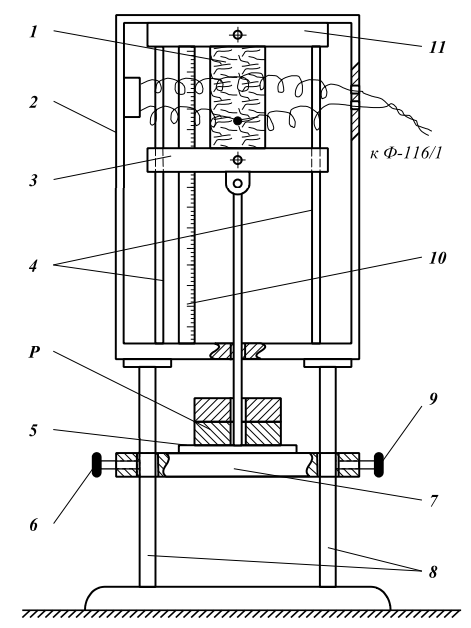
\includegraphics[width=80mm]{schema1.png}
\caption{Схема установки: 1 - образец резины, закреплённый в зажимах 3 и 11, 2 - корпус из оргстекла (нужен для уменьшения флуктуаций температуры), 4 - рейки, по которым может перемещаться зажим 3. 5 - лёгкая подставка для грузов, 6,9 - зажимы для упора 7, который может перемещаться вдоль реек 8. }\label{schema}
\end{figure}

\begin{figure}[ht]
\centering
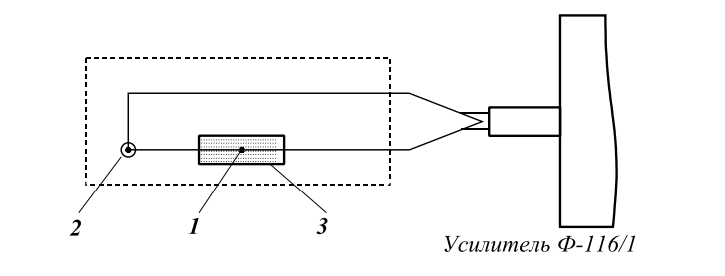
\includegraphics[width=110mm]{schema2.png}
\caption{Схема расположения спаев термопары: 1 - рабочий спай, расположенный внутри резины 3; 2 - компенсирующий спай.}\label{schema}
\end{figure}
\bigskip

Чувствительность термопары - $64 \text{мкВ} / \degree C$. Диаметр проволочек - 0,14 мм.

\bigskip
\newpage
\textbf{Ход работы:}
\bigskip

\textbf{1 Исследование зависимости $f(l), T = const$.}
\medskip

1.1 Снятие зависимости $f(m)$, где $m$ - масса груза при $1 < \lambda < 2,5$. Рекомендуется начать с большого груза. Необходимо выжидать установления температуры.

1.2 Анализ полученных результатов. Определение модуля Юнга для резины.

\textbf{2 Исследование термических эффектов, сопровождающих растяжение.}
\medskip

2.1 Подготовить микровольтметр к работе. ( прогреть, подобрать правильный предел измерения)

2.2 Поместить на платформу груз соотв. $\lambda = 2,5$. Снять зависимость $T(t)$ (t - время).
С помощь экстраполяции получить $T(0)$. Важно растягивать груз не слишком быстро, но достаточно быстро.

2.3 Провести ещё несколько измерений $\lambda = 1,5; 2; 2,5$. Проанализировать результаты. Найти $C_l$.
\bigskip

\textbf{Записи из журнала:}
\bigskip

%
%\bigskip
%
%\textbf{Итог:}
%\bigskip
 
\end{document} % конец документа